\chapter{Data}
\label{ch:DataCommonlyUsedInSpeciesDistributionModels}

\section{Introduction}
To study the performance methods to reduce the number of dimensions in SDMs we need data-sets containing on explanatory and outcome data. The different explanatory variables that are used are described in Section \ref{sec:PredictorData}. Given the goals of the thesis we opted for using $33$ different variables. This is more than used in the average SDM and it should be expected that some of them are quite redundant for the species of interest. The species of interest and data-sets that consist of locations where the species was observed to b present or absent are introduced in Section \ref{sec:OutcomeData}.  \\

To process the spatial data R \parencite{RProg} is used as a geographic information system (GIS). To do this we rely on the \textsc{raster} \parencite{raster} and \textsc{sp} \parencite{sp} packages.
\section{Predictor data}
\label{sec:PredictorData}

\subsection{Vegetation Continuous Fields}
The Vegetation Continuous Fields (\Citeauthor[VCF,][]{VCF}) data-set contains values between $0$ and $100$ which are proportional estimates of the tree cover in the cell. Some cells also contain values larger than $100$ which indicate that the cell contains water or that no data is available. Since R has a \textsc{NA} value all the cells with values larger than $100$ are set to \textsc{NA}. The raster is provided in the geographical coordinate system combined with the World Geodetic System 1984 datum (GCS\textunderscore WGS84). The resolution of the VCF raster is $0.00208$ decimal degrees.

\subsection{Bioclimatic variables}
The bioclimatic variables are a set of variables that describe ecologically relevant climate patterns. \todo[inline]{find a citation} The definition of each of the $19$ bioclimatic variables can be found in Table \ref{table:Bioclim}. The bioclimatic variables can be derived from monthly minimum, maximum, and average temperature and precipitation data. Furthermore, it is clear that the BIO05, BIO6, and BIO7 variables are linear dependent. This linear dependence can be problematic when using classification methods. It is interesting that for some of the methods that we introduce this will lead to no problems while it will for others, see Section \ref{sec:combinations}. \\ 

\begin{table}[htb]
\centering
\begin{tabular}{ll}
\toprule
Variable name & Definition \\ 
\midrule
BIO1 & Annual mean temperature \\
BIO2 & Mean diurnal range (mean of monthly $\left( \text{temp}_{max} - \text{temp}_{min} \right)$) \\
BIO3 & Isothermality $\left( 100 \times \frac{\text{BIO2}}{\text{BIO7}} \right)$  \\
BIO4 & Temperature seasonality $\left(SD(\text{temp}_{avg}) \times 100\right)$ \\
BIO5 & Max temperature of warmest month \\
BIO6 & Min temperature of coldest month \\
BIO7 & Temperature annual range $\left(\text{BIO5} - \text{BIO6}\right)$ \\
BIO8 & Mean temperature of wettest quarter \\
BIO9 & Mean temperature of driest quarter \\
BIO10 & Mean temperature of warmest quarter \\
BIO11 & Mean temperature of coldest quarter \\
BIO12 & Annual precipitation \\
BIO13 & Precipitation of wettest month \\
BIO14 & Precipitation of driest month \\
BIO15 & Precipitation seasonality $\left( \frac{SD( \text{percipitation})}{mean(\text{percipitaiton})} \right)$ \\
BIO16 & Precipitation of wettest quarter \\
BIO17 & Precipitation of driest quarter \\
BIO18 & Precipitation of warmest quarter \\
BIO19 & Precipitation of coldest quarter \\
\bottomrule
\end{tabular}
\caption{\label{table:Bioclim}Definition of the bioclimatic variables.}
\end{table}

The monthly temperature and precipitation data was obtained from the PRISM database (\cite{daly_knowledge-based_2002}, \citeauthor{PRISM}). The PRISM rasters have a grid cell size of $0.00833$ decimal degrees and the rasters are provided in the GCS\textunderscore WGS84 spatial reference system. \\ 

To calculate the bioclimatic variables we adapted the \textsc{biovars} function from the \textsc{dismo} package \parencite{dismo}. The \textsc{biovars} function from the \textsc{dismo} package does not allow the user to provide a layer of the mean temperature. Instead of using the mean temperature in the calculations it uses the average of the minimum and maximum temperature. Our adaptation does use the mean temperature layers and should be slightly more accurate.

\subsection{Normalized Difference Vegetation Index}
The Normalized Difference Vegetation Index (NDVI) is an index of the amount of vegetation. It is based on measurements of the reflectance of the infra-red and the near infra-red region. The NDVI takes on values between $-1$ and $1$. High values correspond with live green vegetation. The NDVI raster used in this thesis originates from the Global Inventory Modelling and Mapping Studies (GIMMS) and is provided by the University of Maryland Global Land Cover Facility \parencite{pinzon2005satellite, tucker2005extended}. This database contains semi-monthly rasters of the NDVI value for the period 1983-2006. The original rasters had a cell-size of $0.07266$ decimal degrees. These rasters were originally \todo[inline]{cite paper Brody / Svenning on greenes in the US} resampled to $0.04166$ decimal degree rasters and cells with values corresponding to water or with no data available were set to \textsc{NA}. The semi-monthly rasters were then combined such that monthly rasters were obtained. To obtain an average monthly NDVI raster for each month the $24$ NDVI rasters of the different years were averaged. The $12$ resulting monthly NDVI rasters can then be used to calculate a minimum, maximum, and mean NDVI raster.

\subsection{Digital elevation model}
The digital elevation model (DEM) raster \parencite{DEM} contains data on the elevation throughout the US. It is the raster with the highest resolution, more specifically the cell size is $0.000833$ decimal degrees and the raster is provided in the GCS\textunderscore WGS84 spatial reference system. The use of elevation data in SDM is somewhat contested, see e.g.\ \cite{hof_usefulness_2012} and \cite{oke_distribution_2015}. However, since our main purpose is to test model selection techniques adding a potentially irrelevant predictor should not matter. Furthermore, it is often suggested that other variables directly derived from DEMs, e.g.\ slope, are more ecological relevant \parencite{franklin_mapping_2009}. However, to keep the amount of data in this thesis handleable we will restrict ourselves to the original DEM raster.


\subsection{Land cover}
The land cover data was created from the National Land Cover Databases (NLCD) provided by the US Geological Survey. The NLCD were derived from landsat imagery of 2001 \parencite{vogelmann2001completion}, 2007 \parencite{homer2007completion}, and 2011 \parencite{fry2011completion}. These datasets were then transformed into rasters that utilize the Anderson level 1 classification \parencite{anderson_land_1976}. Eight different land cover classes are used: barren, forest, ice-snow, grassland, urban, water, wetlands, agriculture. For each land cover class-year combination rasters with a cell size of $0.04166$ decimal degrees were created. In order to obtain one raster for each land cover class the three corresponding rasters were averaged. The eight final rasters were then rescaled such that the values of the rasters lie within the interval $[0,1]$. For each land cover class raster the cell values are an estimate of the percentage of the land of this class within the cell. It is interesting that the sum of these rasters equals one, hence there is a linear dependence between the variables.

\subsection{Human Influence Index}
The Human Influence Index (\citeauthor{hii}) raster contains integer values between $0$ and $64$. High values indicate a strong human influence and vice versa. The index is derived from measures of the population density, the amount of roads, the amount of light sources during night-time, etc. The raster is reprojected to the GCS\textunderscore WGS84 spatial reference system and has a cell size of $0.00833$ decimal degrees.

\subsection{Preprocessing of the predictor data}

In order to speed up computations and facilitate general GIS operations the rasters were, if necessary, reprojected to the GCS\textunderscore WGS84 spatial reference system. The extent and resolution of the rasters was set to be equal to those of the DEM layer. When it was necessary bilinear interpolation was used. This procedure makes sure that the cells of the rasters line up nicely. A visualization of the whole process can be found in Figure \ref{fig:DataCommonlyUsedInSpeciesDistributionModels:DataScheme}. Once all the data was preprocessed the rasters amount to over $300$ GB of data.

\begin{figure}[!htb]
\centering
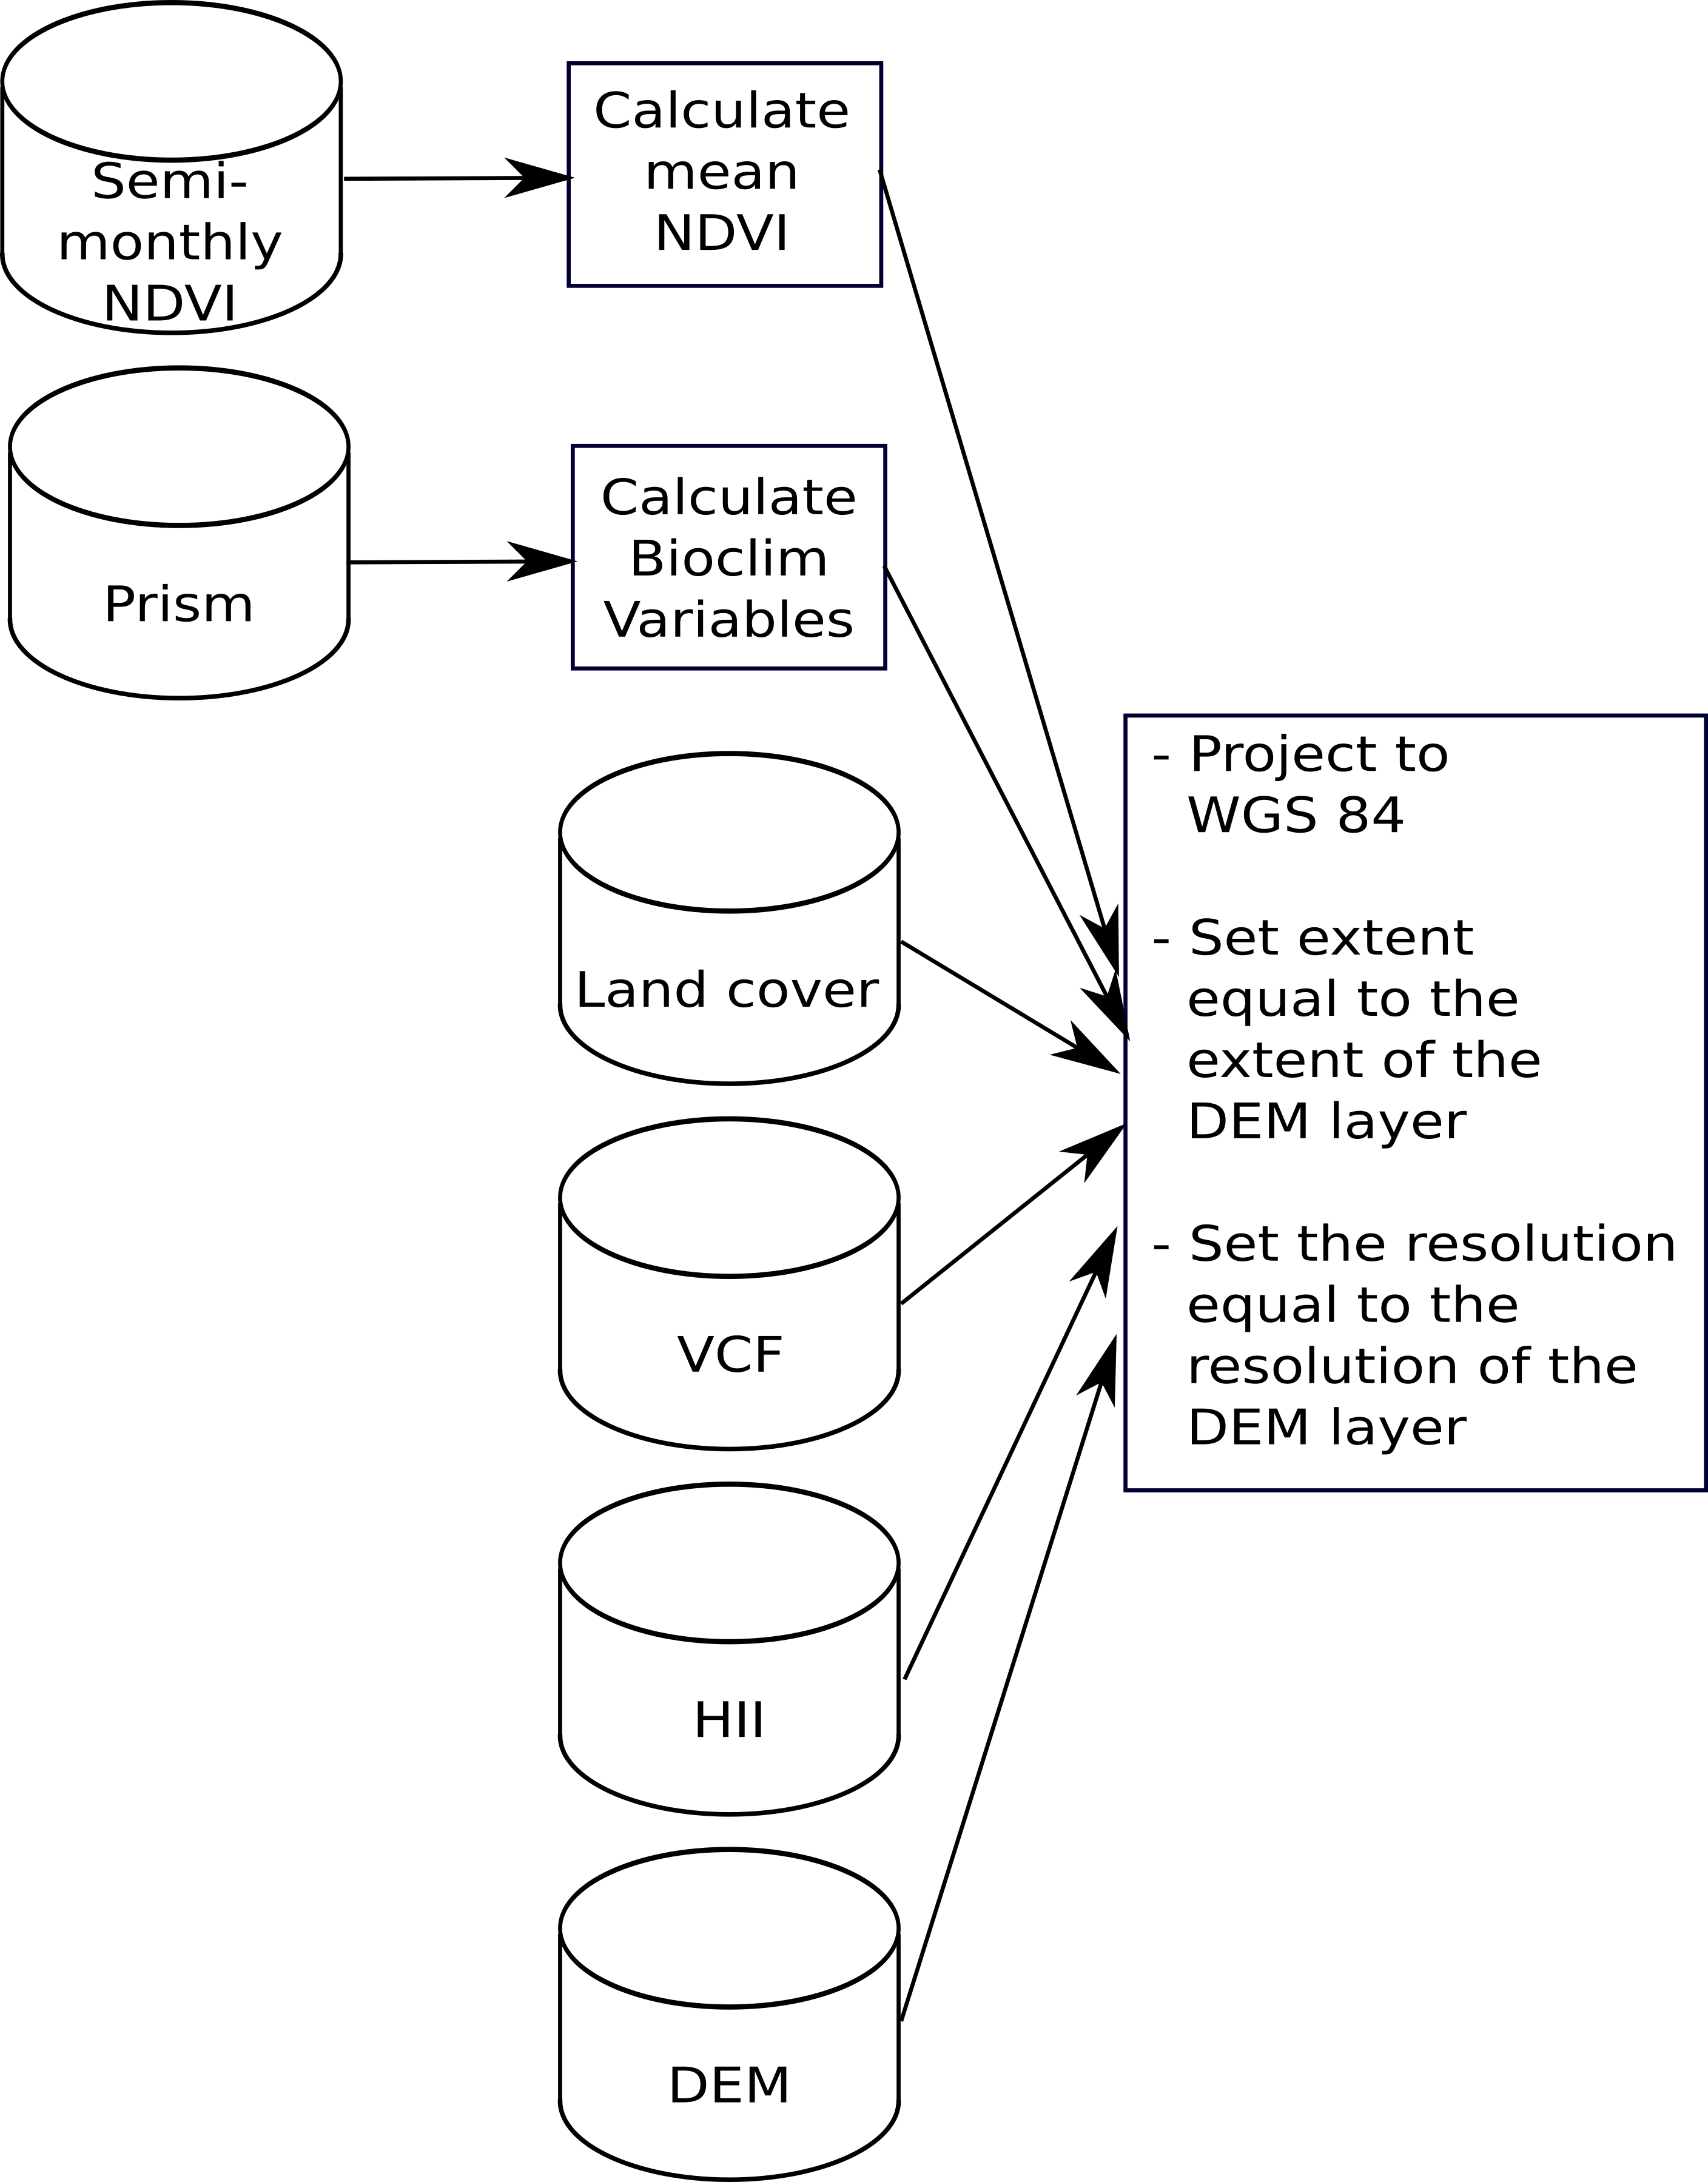
\includegraphics[scale=0.35]{VectorGraphics/DataScheme.png}
\caption{\label{fig:DataCommonlyUsedInSpeciesDistributionModels:DataScheme}Visualization of the preprocessing of the raster data.}
\end{figure}


\subsection{Exploratory analysis of the predictor data}
\label{sec:ExploratoryPredictor}
It might be expected that the relationship between the variables is different in different regions of the contiguous US. To test this we defined four regions, their bounding rectangles can be found in Figure \ref{fig:studyExtent}. To test our suspicions two sets of random points were generated: one with points within the contiguous United States and one that contains points within the West Coast region. For each point the corresponding values of the predictor rasters were extracted. Heat maps of the correlations of the predictor variables can be found in Figures \ref{fig:HeatBGUS} and \ref{fig:HeatBGWC}. A quick inspection of these plots learns that most correlations are approximately equal in the two ranges. There are also some correlations that change quite dramatically, e.g.\ the correlation between the ice-snow land cover class and the NDVI indices. Even though we only report the heat maps of the correlations for the US and the West Coast region similar similar changes can be observed for the other regions. \\

\begin{figure}[!htb]
\centering
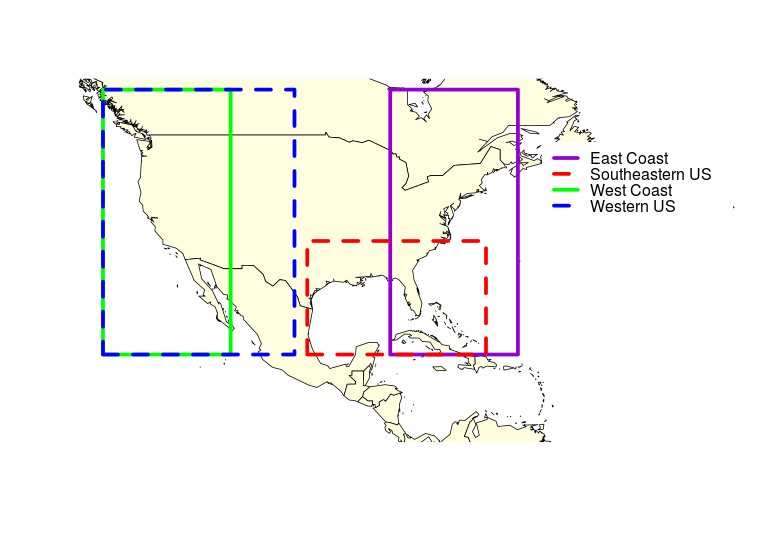
\includegraphics[scale=0.6]{Plots/StudyExtent.png}
\caption{\label{fig:studyExtent}Regions of the contiguous US and their bounding rectangles.}
\end{figure}


\begin{landscape}
\thispagestyle{empty}
\null
\vskip 0.6cm

\begin{figure}[!htb]
  \centering
  \makebox[\textwidth][c]{%
    \begin{minipage}{.90\textwidth}
    \centering
    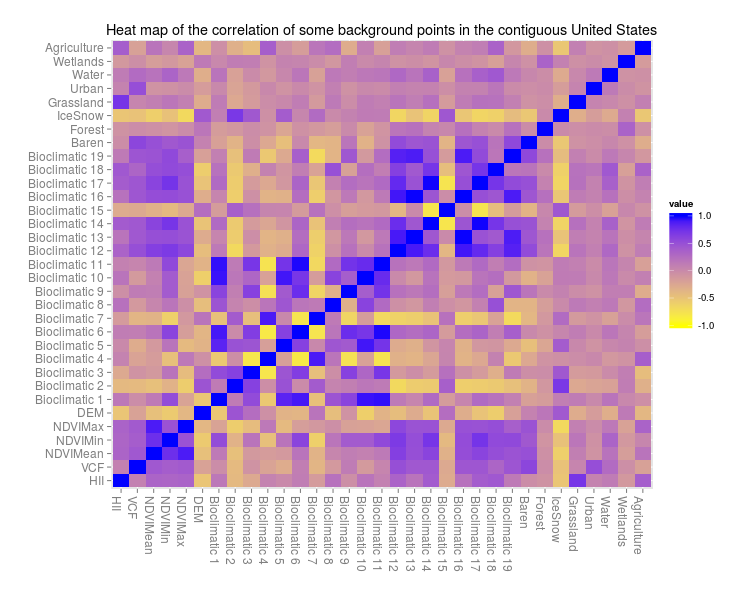
\includegraphics[width=\textwidth]{Plots/CorPlotUS.png}
    \caption{\label{fig:HeatBGUS}Heat map of the correlations in the contiguous US.}
    \end{minipage}
    \begin{minipage}{.90\textwidth}
    \centering
    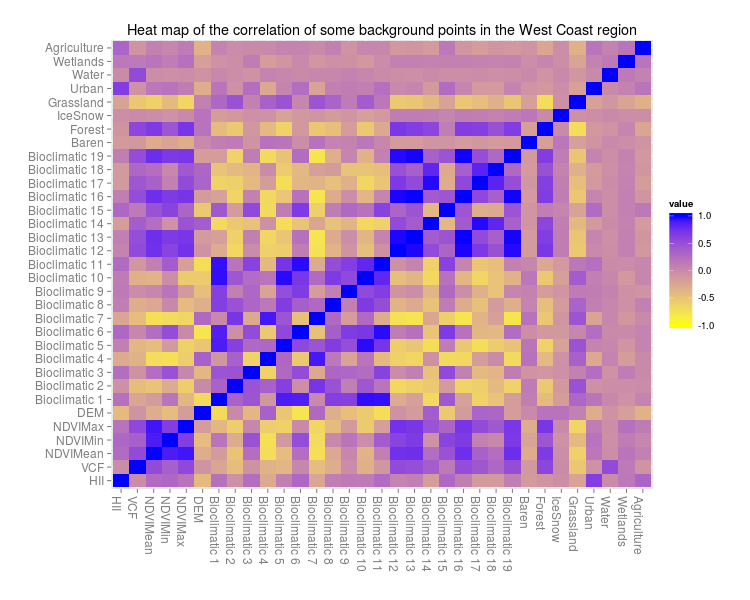
\includegraphics[width=\textwidth]{Plots/CorPlotBGWC.png}
    \caption{\label{fig:HeatBGWC}Heat map of the correlations in the West Coast region.}		\end{minipage}%
}
\end{figure}
\end{landscape}

It is interesting to note that the rank of the predictor data matrix of the random points is $32$. This is rather surprising since BIO7 is a linear combination of BIO5 and BIO6 and the land cover variables should sum to a constant. Hence one would expect that the rank is smaller or equal to $33-2 =31$. A closer inspection leads to the conclusion that some small rounding errors in the creation of the land cover rasters ``remove'' the linear dependence. This ``near linear dependence'' also becomes clear when we look at the singular values of the scaled data matrix. The three smallest are $0.2139771, 0.000002,$ and $0$, for all practical purposes this means that there are two redundant variables.\\

\section{Outcome data}
\label{sec:OutcomeData}
\subsection{Species considered}
The species that will be studied can be found in Table \ref{table:Species}. These species were selected so that different regions in the US are represented. This was done because, as we saw in Section \ref{sec:ExploratoryPredictor}, the relationship between the different predictors can be different in different regions. The extent of the species distribution is quite different across the selected species. For example, the copperhead snake is spread throughout a large part of the US while the Sequoia sempervirens only occurs in a small strip of land stretching from Southern California to Southern Oregon. Finally, the selected species consist of five plant and five animal species. Selecting both plant and animal species was done because it seems reasonable that the including fine grain predictors will lead to a larger increase in predictive performance of the classification models when the species is stationary.\\

\begin{sidewaystable}[!htb]
\centering
\begin{tabular}{l l c c c c c }
\toprule
Species & Common name & US & West Coast & East Coast & Western US & Southeastern US \\
\midrule
Aesculus glabra & Ohio buckeye  &  \ding{51} \\
Juniperus osteosperma & Utah juniper  & & &  \ding{51}\\
Quercus ilicifolia & bear oak  & & &  \ding{51}  \\
Salix caroliniana & coastal plain willow  &  \ding{51}  \\
Sequoia sempervirens & coast redwood & &  \ding{51}  \\
\\
Agkistrodon contortrix Linnaeus & copperhead snake   &  \ding{51}  \\
Geomys pinetis Rafinesque & southeastern pocket gopher  &&&& &  \ding{51}  \\
Pituophis catenifer catenifer & Pacific gopher snake  &  &  \ding{51}  \\
Sorex pacificus & Pacific shrew &  &  \ding{51}  \\
Sylvilagus nuttallii & mountain cottontail  & & &  &  \ding{51}  \\
\bottomrule
\end{tabular}
\caption{\label{table:Species}The different species studied and their study extent.}
\end{sidewaystable}

\subsection{Global Biodiversity Information Facility}
The presence-only data originates from the Global Biodiversity Information Facility (GBIF) database. This database contains data from other smaller presence-only databases. Examples include data from citizen science projects (e.g.\ the iNaturalist project) or herbariums (e.g.\ The New York Botanical Garden Herbarium). These data sources are quite prone to errors. Citizen science data is usually provided by non-experts and misidentifications are quite likely. Even data collected by experts can be irrelevant for our purposes, for example herbarium data often includes specimens located inside botanical gardens etc. GBIF data tends to contain a lot of duplicated observations. Hence, before using the data from GBIF some data-cleaning was performed. Finally, because the predictors were recorded quite recently we decided to restrict ourselves to observations obtained from the 1980s onward. This somewhat prevents the situation where the current predictor values have changed recently, e.g. due to deforestation.\\
\todo[inline]{change this sentence}X

\subsection{Forest Inventory and Analysis data}
The presence-absence data of the plant species was obtained from the The United States Forest Service Forest Inventory and Analysis (FIA) database. The data from this database consists of plot locations and all the tree species observed within each plot are recorded. The reported coordinates of the plots are, for privacy reasons, slightly distorted.\\ 

The sampling design that is used in the construction of this database changed in 1999 and details can be found in \cite{fiamanual}. By 2004 the new sampling design was implemented in nearly all the states of the contiguous US. The exceptions to this are New Mexico, Oklahoma, and Wyoming for which the new design was implemented in 2005, 2008-2009, and 2011. In each state at least $10\%$ of the plots are sampled each year. By using a time-frame of $10$ years we ensure that each plot site was sampled. More particularly, the time-frame that we use is 2004-2014. Since the sampling in New Mexico, Oklahoma, and Wyoming started later than 2004 these states are under-sampled. States in the Eastern US tend to have a sample intensity larger than $10\%$ and some plots were sampled multiple times. Plots that were sampled multiple times were replaced by new observations. If a plot contained the species of interest at least once the species is said to have been present, otherwise it was absent in the plot. It might be interesting to use modelling methods that allow for a sampling design correction. However, this would lead us astray and the sampling design will not be corrected for in this thesis.\\

Finally, all of the sampled plots are contained within forested areas. This implies that lone standing trees were not observed.

\subsection{Data preparation}
In order to build the necessary models the predictor values corresponding to the presence or absence locations need to be extracted. For certain locations some of the rasters contain a \textsc{NA} value. These locations were removed before the models were constructed.
\section{Spatial scale}
\label{sec:SpatialScale}

\todo[inline]{cite Fine-scale environmental variation in species distribution modelling ...}